% !TEX program = xelatex
\documentclass[12pt,a4paper]{article}

\usepackage{fontspec}
\usepackage{polyglossia}
\setmainlanguage{greek}
\setotherlanguage{english}
\setmainfont[Script=Greek]{DejaVu Serif}
\setsansfont[Script=Greek]{DejaVu Sans}
\setmonofont[Script=Greek]{DejaVu Sans Mono}
\newfontfamily\greekfonttt[Script=Greek]{DejaVu Sans Mono}

\usepackage[a4paper, margin=2.4cm]{geometry}
\usepackage{amsmath, amssymb}
\usepackage{booktabs}
\usepackage{array}
\usepackage{longtable}
\usepackage{graphicx}
\usepackage{float}
\usepackage{caption}
\usepackage{subcaption}
\usepackage[hidelinks]{hyperref}
\usepackage{enumitem}
\usepackage{parskip}
\usepackage{xcolor}
\usepackage{fancyhdr}

\pagestyle{fancy}
\fancyhf{}
\lhead{Ανάλυση Δεδομένων 2025--26}
\rhead{4η Εργασία -- ΑΕΜ 6931}
\cfoot{\thepage}
\setlength{\headheight}{14.5pt}

\newcommand{\code}[1]{\texttt{\textenglish{#1}}}
\newcommand{\acc}{\textenglish{accuracy}}
\newcommand{\te}{\textenglish{test error}}

\title{
    \textbf{Ανάλυση Δεδομένων 2025--26}\\[0.25cm]
    \Large 4η Εργασία: Μέθοδοι Δέντρων και Συνόλων Ταξινομητών\\[0.15cm]
    \large Πρόβλεψη τύπου κρασιού με Decision Tree, Bagging, Random Forest και Boosting
}
\author{
    Ρακοβαλής Παύλος\\
    ΑΕΜ: 6931
}
\date{\today}

\begin{document}

\maketitle
\thispagestyle{fancy}

\begin{abstract}
Στην παρούσα εργασία χρησιμοποιούνται τα δεδομένα της 3ης εργασίας με στόχο
την πρόβλεψη του τύπου κρασιού, δηλαδή αν ένα κρασί είναι λευκό ή κόκκινο.
Ως προβλεπτικές μεταβλητές χρησιμοποιούνται όλα τα φυσικοχημικά
χαρακτηριστικά εκτός από τη μεταβλητή \code{quality}. Εφαρμόζονται τέσσερις
μέθοδοι ταξινόμησης: δέντρο ταξινόμησης, Bagging, Random Forest και Boosting.
Αρχικά αξιολογούνται τα μοντέλα με τις υπερπαραμέτρους που ζητούνται στην
εκφώνηση και στη συνέχεια μελετάται η επίδραση του βάθους του δέντρου και του
αριθμού εκτιμητών. Τέλος, πραγματοποιείται βελτιστοποίηση υπερπαραμέτρων με
Grid Search και 5-fold stratified cross-validation. Τα αποτελέσματα δείχνουν
ότι όλες οι ensemble μέθοδοι έχουν πολύ υψηλή ακρίβεια, ενώ το καλύτερο
βελτιστοποιημένο μοντέλο είναι το Bagging με test accuracy 0.9729.
\end{abstract}

\tableofcontents
\newpage

%=============================================================================
\section{Εισαγωγή και περιγραφή δεδομένων}
%=============================================================================

Στόχος της 4ης εργασίας είναι η εκτίμηση του τύπου κρασιού
(\code{wine\_type}), δηλαδή η ταξινόμηση κάθε παρατήρησης ως λευκό
(\code{white}) ή κόκκινο (\code{red}) κρασί. Για την ανάλυση χρησιμοποιούνται
τα δεδομένα της 3ης εργασίας. Το αρχικό αρχείο περιλαμβάνει $5\,295$
παρατηρήσεις και 13 μεταβλητές: 11 φυσικοχημικά χαρακτηριστικά, τη μεταβλητή
\code{quality} και τη μεταβλητή στόχο \code{wine\_type}.

Σύμφωνα με την εκφώνηση, η μεταβλητή \code{quality} δεν χρησιμοποιείται ως
προβλεπτική μεταβλητή. Άρα το πλήθος των προβλεπτικών μεταβλητών είναι
$p=11$:

\begin{center}
\footnotesize
\begin{tabular}{lll}
\toprule
\code{fixed acidity} & \code{volatile acidity} & \code{citric acid} \\
\code{residual sugar} & \code{chlorides} & \code{free sulfur dioxide} \\
\code{total sulfur dioxide} & \code{density} & \code{pH} \\
\code{sulphates} & \code{alcohol} & \\
\bottomrule
\end{tabular}
\end{center}

Η μεταβλητή απόκρισης κωδικοποιήθηκε ως:
\begin{center}
    \code{red = 0} \hspace{1cm} και \hspace{1cm} \code{white = 1}.
\end{center}

Η κατανομή των κλάσεων στο σύνολο δεδομένων είναι:

\begin{table}[H]
\centering
\caption{Κατανομή της μεταβλητής \code{wine\_type}.}
\begin{tabular}{lrr}
\toprule
\textbf{Κλάση} & \textbf{Πλήθος} & \textbf{Ποσοστό} \\
\midrule
\code{white} & 3991 & 75.37\% \\
\code{red}   & 1304 & 24.63\% \\
\bottomrule
\end{tabular}
\end{table}

Παρατηρείται ότι οι κλάσεις δεν είναι ισορροπημένες, καθώς τα λευκά κρασιά
είναι περίπου τριπλάσια από τα κόκκινα. Για τον λόγο αυτό, ο διαχωρισμός σε
training και test έγινε με \code{stratify=y}, ώστε να διατηρηθεί περίπου η ίδια
αναλογία κλάσεων και στα δύο υποσύνολα.

Σε όλα τα ερωτήματα χρησιμοποιήθηκε διαχωρισμός:
\[
    70\% \text{ training set}, \qquad 30\% \text{ test set}.
\]
Το \code{random\_state} τέθηκε ίσο με τον ΑΕΜ:
\begin{center}
    \code{random\_state = 6931}.
\end{center}

Έτσι προέκυψαν:
\[
    n_{\text{train}}=3706, \qquad n_{\text{test}}=1589.
\]
Στο test set υπάρχουν 391 κόκκινα και 1198 λευκά κρασιά.

\subsection{Κριτήριο αξιολόγησης}

Για κάθε μοντέλο υπολογίζεται η ακρίβεια στο test set:
\[
    \text{Test Accuracy} =
    \frac{\text{αριθμός σωστών προβλέψεων}}{\text{σύνολο παρατηρήσεων test}}.
\]

Επίσης, σύμφωνα με τα ερωτήματα 5 και 6, χρησιμοποιείται το test error:
\[
    \text{Test Error} = 1 - \text{Test Accuracy}.
\]

Οι πίνακες σύγχυσης παρουσιάζονται με γραμμές τις πραγματικές κλάσεις και
στήλες τις προβλεπόμενες κλάσεις:

\begin{center}
\begin{tabular}{lcc}
\toprule
& \textbf{pred red} & \textbf{pred white} \\
\midrule
\textbf{true red} & TN & FP \\
\textbf{true white} & FN & TP \\
\bottomrule
\end{tabular}
\end{center}

%=============================================================================
\section{Ερώτημα 1: Δέντρο ταξινόμησης μέγιστου βάθους 2}
%=============================================================================

Στο πρώτο ερώτημα εφαρμόστηκε δέντρο ταξινόμησης με μέγιστο βάθος 2. Το μοντέλο
που χρησιμοποιήθηκε ήταν:

\begin{center}
\small
\code{DecisionTreeClassifier(max\_depth=2, random\_state=6931)}
\end{center}

Το μικρό βάθος περιορίζει την πολυπλοκότητα του μοντέλου. Έτσι το δέντρο είναι
εύκολα ερμηνεύσιμο, αλλά πιθανόν να μην μπορεί να αποτυπώσει όλες τις
σύνθετες σχέσεις μεταξύ των μεταβλητών και της κλάσης.

\subsection{Αποτελέσματα}

\begin{table}[H]
\centering
\caption{Αποτελέσματα δέντρου ταξινόμησης με \code{max\_depth=2}.}
\begin{tabular}{lrrrr}
\toprule
\textbf{Μοντέλο} & \textbf{max depth} & \textbf{Test Accuracy} & \textbf{Test Error} & \textbf{Λάθη} \\
\midrule
Decision Tree & 2 & 0.9339 & 0.0661 & 105 \\
\bottomrule
\end{tabular}
\end{table}

\begin{table}[H]
\centering
\caption{Πίνακας σύγχυσης για το δέντρο ταξινόμησης.}
\begin{tabular}{lcc}
\toprule
& \textbf{pred red} & \textbf{pred white} \\
\midrule
\textbf{true red}   & 360 & 31 \\
\textbf{true white} & 74  & 1124 \\
\bottomrule
\end{tabular}
\end{table}

Το μοντέλο ταξινόμησε σωστά $360+1124=1484$ από τις $1589$ παρατηρήσεις του
test set. Η τελική ακρίβεια είναι:
\[
    \frac{1484}{1589}=0.9339.
\]

\subsection{Ερμηνεία του δέντρου}

Οι κανόνες που προέκυψαν από το δέντρο είναι:

\begin{verbatim}
total sulfur dioxide <= 67.50
|-- chlorides <= 0.05  -> white
|-- chlorides >  0.05  -> red

total sulfur dioxide > 67.50
|-- chlorides <= 0.07  -> white
|-- chlorides >  0.07  -> red
\end{verbatim}

Άρα, για βάθος 2, το δέντρο βασίζεται κυρίως σε δύο μεταβλητές:
\code{total sulfur dioxide} και \code{chlorides}. Αυτό είναι λογικό για το
συγκεκριμένο πρόβλημα, καθώς τα λευκά και τα κόκκινα κρασιά συχνά διαφέρουν
αρκετά στις τιμές των θειωδών και των χλωριδίων. Παρά την απλότητά του, το
μοντέλο πετυχαίνει πολύ καλή ακρίβεια, περίπου 93.39\%.

%=============================================================================
\section{Ερώτημα 2: Bagging με 200 εκτιμητές}
%=============================================================================

Στο δεύτερο ερώτημα εφαρμόστηκε η μέθοδος Bagging
(\textenglish{Bootstrap Aggregating}). Η βασική ιδέα της μεθόδου είναι ότι
εκπαιδεύονται πολλά δέντρα ταξινόμησης σε διαφορετικά bootstrap δείγματα του
training set και η τελική πρόβλεψη προκύπτει με πλειοψηφική ψηφοφορία.

Το μοντέλο που χρησιμοποιήθηκε ήταν:

\begin{center}
\small
\code{BaggingClassifier(estimator=DecisionTreeClassifier(), n\_estimators=200, random\_state=6931)}
\end{center}

Σε αντίθεση με το απλό δέντρο του ερωτήματος 1, εδώ δεν χρησιμοποιείται μόνο
ένα δέντρο, αλλά σύνολο 200 δέντρων. Αυτό μειώνει τη διακύμανση της πρόβλεψης,
καθώς τα λάθη μεμονωμένων δέντρων τείνουν να εξομαλύνονται μέσω της
ψηφοφορίας.

\subsection{Αποτελέσματα}

\begin{table}[H]
\centering
\caption{Αποτελέσματα Bagging με 200 εκτιμητές.}
\begin{tabular}{lrrrr}
\toprule
\textbf{Μοντέλο} & \textbf{n estimators} & \textbf{Test Accuracy} & \textbf{Test Error} & \textbf{Λάθη} \\
\midrule
Bagging & 200 & 0.9660 & 0.0340 & 54 \\
\bottomrule
\end{tabular}
\end{table}

\begin{table}[H]
\centering
\caption{Πίνακας σύγχυσης για το Bagging.}
\begin{tabular}{lcc}
\toprule
& \textbf{pred red} & \textbf{pred white} \\
\midrule
\textbf{true red}   & 365 & 26 \\
\textbf{true white} & 28  & 1170 \\
\bottomrule
\end{tabular}
\end{table}

Το Bagging ταξινόμησε σωστά $365+1170=1535$ από τις $1589$ παρατηρήσεις.
Η ακρίβεια αυξήθηκε από 0.9339 στο απλό δέντρο σε 0.9660, ενώ το test error
μειώθηκε από 0.0661 σε 0.0340.

\subsection{Σχόλιο}

Η βελτίωση σε σχέση με το απλό δέντρο είναι σημαντική. Το απλό δέντρο
περιορίζεται σε λίγους κανόνες, ενώ το Bagging συνδυάζει πολλά δέντρα και
μειώνει την αστάθεια που χαρακτηρίζει τα δέντρα απόφασης. Επομένως, η μέθοδος
πετυχαίνει καλύτερη γενίκευση στο test set.

%=============================================================================
\section{Ερώτημα 3: Random Forest με 200 εκτιμητές και \texorpdfstring{$m=p/2$}{m=p/2}}
%=============================================================================

Στο τρίτο ερώτημα εφαρμόστηκε Random Forest. Η μέθοδος είναι επέκταση του
Bagging, με τη διαφορά ότι σε κάθε split κάθε δέντρου δεν εξετάζονται όλες οι
μεταβλητές, αλλά ένα τυχαίο υποσύνολό τους. Αυτό μειώνει τη συσχέτιση μεταξύ
των δέντρων και συχνά οδηγεί σε καλύτερη απόδοση.

Στην παρούσα εργασία το πλήθος των προβλεπτικών μεταβλητών είναι:
\[
    p=11.
\]
Η εκφώνηση ζητά τυχαίο πλήθος υποψήφιων χαρακτηριστικών:
\[
    m = \frac{p}{2} = 5.5.
\]
Επειδή στο \code{scikit-learn} το \code{max\_features} πρέπει να είναι
ακέραιος αριθμός όταν δηλώνεται ως πλήθος μεταβλητών, χρησιμοποιήθηκε:
\[
    m=5.
\]

Το μοντέλο ήταν:

\begin{center}
\small
\code{RandomForestClassifier(n\_estimators=200, max\_features=5, random\_state=6931)}
\end{center}

\subsection{Αποτελέσματα}

\begin{table}[H]
\centering
\caption{Αποτελέσματα Random Forest.}
\begin{tabular}{lrrrrr}
\toprule
\textbf{Μοντέλο} & \textbf{n estimators} & \textbf{p} & \textbf{m} & \textbf{Test Accuracy} & \textbf{Test Error} \\
\midrule
Random Forest & 200 & 11 & 5 & 0.9666 & 0.0334 \\
\bottomrule
\end{tabular}
\end{table}

\begin{table}[H]
\centering
\caption{Πίνακας σύγχυσης για το Random Forest.}
\begin{tabular}{lcc}
\toprule
& \textbf{pred red} & \textbf{pred white} \\
\midrule
\textbf{true red}   & 365 & 26 \\
\textbf{true white} & 27  & 1171 \\
\bottomrule
\end{tabular}
\end{table}

Το Random Forest ταξινόμησε σωστά $365+1171=1536$ παρατηρήσεις και έκανε 53
λάθη. Η ακρίβεια ήταν 0.9666, δηλαδή ελαφρώς υψηλότερη από εκείνη του
Bagging.

\subsection{Σχόλιο}

Η διαφορά Random Forest και Bagging είναι μικρή στο συγκεκριμένο πρόβλημα.
Ωστόσο, το Random Forest έχει ένα θεωρητικό πλεονέκτημα: επειδή κάθε split
εξετάζει μόνο τυχαίο υποσύνολο μεταβλητών, τα δέντρα του ensemble είναι
λιγότερο συσχετισμένα μεταξύ τους. Αυτό μπορεί να μειώσει περαιτέρω τη
διακύμανση του τελικού μοντέλου. Στα συγκεκριμένα δεδομένα, η βελτίωση είναι
οριακή αλλά υπαρκτή.

%=============================================================================
\section{Ερώτημα 4: Boosting με 200 επιμέρους μοντέλα}
%=============================================================================

Στο τέταρτο ερώτημα εφαρμόστηκε Boosting με 200 επιμέρους μοντέλα,
συντελεστή μάθησης 0.1 και μέγιστο βάθος 1. Χρησιμοποιήθηκε ο ταξινομητής
\code{GradientBoostingClassifier}, ο οποίος κατασκευάζει διαδοχικά ασθενή
μοντέλα, όπου κάθε νέο μοντέλο προσπαθεί να διορθώσει τα λάθη των προηγούμενων.

Το μοντέλο ήταν:

\begin{center}
\small
\code{GradientBoostingClassifier(n\_estimators=200, learning\_rate=0.1, max\_depth=1, random\_state=6931)}
\end{center}

Το \code{max\_depth=1} σημαίνει ότι κάθε επιμέρους μοντέλο είναι δέντρο
βάθους 1, δηλαδή decision stump. Κάθε τέτοιο δέντρο είναι πολύ απλό, αλλά ο
συνδυασμός πολλών τέτοιων μοντέλων μπορεί να οδηγήσει σε ισχυρό ταξινομητή.

\subsection{Αποτελέσματα}

\begin{table}[H]
\centering
\caption{Αποτελέσματα Boosting.}
\begin{tabular}{lrrrr}
\toprule
\textbf{Μοντέλο} & \textbf{n estimators} & \textbf{learning rate} & \textbf{max depth} & \textbf{Test Accuracy} \\
\midrule
Boosting & 200 & 0.1 & 1 & 0.9679 \\
\bottomrule
\end{tabular}
\end{table}

\begin{table}[H]
\centering
\caption{Πίνακας σύγχυσης για το Boosting.}
\begin{tabular}{lcc}
\toprule
& \textbf{pred red} & \textbf{pred white} \\
\midrule
\textbf{true red}   & 361 & 30 \\
\textbf{true white} & 21  & 1177 \\
\bottomrule
\end{tabular}
\end{table}

Το Boosting ταξινόμησε σωστά $361+1177=1538$ παρατηρήσεις και έκανε 51 λάθη.
Η ακρίβεια του μοντέλου ήταν 0.9679 και το test error 0.0321.

\subsection{Σχόλιο}

Μεταξύ των αρχικών μοντέλων των ερωτημάτων 1--4, το Boosting έχει την
υψηλότερη ακρίβεια. Η μέθοδος φαίνεται να αξιοποιεί αποτελεσματικά τους
ασθενείς ταξινομητές βάθους 1, καθώς κάθε επόμενος ταξινομητής βελτιώνει
σταδιακά τις προηγούμενες προβλέψεις. Ιδιαίτερα αξιοσημείωτο είναι ότι το
Boosting έκανε μόνο 21 λάθος ταξινομήσεις λευκών κρασιών ως κόκκινα, δηλαδή
λιγότερες από τις αντίστοιχες μεθόδους Bagging και Random Forest.

%=============================================================================
\section{Ερώτημα 5: Test error του δέντρου ως συνάρτηση του βάθους}
%=============================================================================

Στο πέμπτο ερώτημα μελετήθηκε η επίδραση του μέγιστου βάθους του δέντρου
ταξινόμησης στο test error. Για τον σκοπό αυτό εκπαιδεύτηκαν δέντρα με
\code{max\_depth} από 1 έως 20.
Για κάθε τιμή του βάθους υπολογίστηκε η ακρίβεια στο ίδιο test set και στη
συνέχεια το test error:
\[
    \text{Test Error} = 1 - \text{Test Accuracy}.
\]

\subsection{Αριθμητικά αποτελέσματα}

\begin{table}[H]
\centering
\caption{Test accuracy και test error για διαφορετικά βάθη δέντρου.}
\small
\begin{tabular}{rrr|rrr}
\toprule
\textbf{Depth} & \textbf{Accuracy} & \textbf{Error} &
\textbf{Depth} & \textbf{Accuracy} & \textbf{Error} \\
\midrule
1  & 0.9119 & 0.0881 & 11 & 0.9610 & 0.0390 \\
2  & 0.9339 & 0.0661 & 12 & 0.9497 & 0.0503 \\
3  & 0.9509 & 0.0491 & 13 & 0.9497 & 0.0503 \\
4  & 0.9629 & 0.0371 & 14 & 0.9484 & 0.0516 \\
5  & 0.9641 & 0.0359 & 15 & 0.9465 & 0.0535 \\
6  & 0.9654 & 0.0346 & 16 & 0.9396 & 0.0604 \\
7  & 0.9616 & 0.0384 & 17 & 0.9408 & 0.0592 \\
8  & 0.9616 & 0.0384 & 18 & 0.9415 & 0.0585 \\
9  & 0.9604 & 0.0396 & 19 & 0.9358 & 0.0642 \\
10 & 0.9597 & 0.0403 & 20 & 0.9346 & 0.0654 \\
\bottomrule
\end{tabular}
\end{table}

\begin{figure}[H]
\centering

\includegraphics[width=0.88\textwidth]{q5_tree_depth_error.png}
\caption{Test error του δέντρου ταξινόμησης συναρτήσει του μέγιστου βάθους.}
\label{fig:q5-depth-error}
\end{figure}

\subsection{Σχολιασμός}

Για πολύ μικρά βάθη, το δέντρο είναι υπερβολικά απλό. Για παράδειγμα, στο
\code{max\_depth=1} το test error είναι 0.0881, ενώ στο
\code{max\_depth=2} μειώνεται σε 0.0661. Αυτό δείχνει ότι το πολύ ρηχό δέντρο
δεν έχει αρκετή ευελιξία ώστε να διαχωρίσει ικανοποιητικά τις δύο κλάσεις.

Καθώς το βάθος αυξάνεται από 1 έως 6, το test error μειώνεται συνεχώς. Η
καλύτερη τιμή εμφανίζεται στο \code{max\_depth=6}, όπου:
\[
    \text{Test Accuracy}=0.9654, \qquad
    \text{Test Error}=0.0346.
\]

Μετά το βάθος 6, το test error δεν συνεχίζει να μειώνεται. Αντίθετα,
παρουσιάζει γενικά ανοδική τάση, ιδιαίτερα για βάθη μεγαλύτερα από 11. Αυτό
είναι ένδειξη πιθανής υπερπροσαρμογής: το δέντρο γίνεται πολύ σύνθετο,
προσαρμόζεται περισσότερο στις ιδιαιτερότητες του training set και χάνει μέρος
της ικανότητας γενίκευσης στο test set.

Συνεπώς, ένα μέτριο βάθος δέντρου είναι καταλληλότερο από ένα πολύ ρηχό ή ένα
πολύ βαθύ δέντρο. Το αποτέλεσμα αυτό συμφωνεί και με το tuning του ερωτήματος
7, όπου το βέλτιστο βάθος για το δέντρο ταξινόμησης επιλέχθηκε επίσης ίσο με
6.

%=============================================================================
\section{Ερώτημα 6: Test error των ensemble μεθόδων ως συνάρτηση του \texorpdfstring{\code{n\_estimators}}{n estimators}}
%=============================================================================

Στο έκτο ερώτημα μελετήθηκε η επίδραση του αριθμού των εκτιμητών στο test
error των τριών ensemble μεθόδων:

\begin{itemize}[nosep]
    \item Bagging,
    \item Random Forest,
    \item Boosting.
\end{itemize}

Οι τιμές που εξετάστηκαν ήταν \code{n\_estimators=1, 10, 20, ..., 200}.

Για κάθε μέθοδο και για κάθε τιμή του \code{n\_estimators} εκπαιδεύτηκε νέο
μοντέλο στο ίδιο training set και υπολογίστηκε το test error στο ίδιο test set.

\subsection{Αριθμητικά αποτελέσματα}

\begin{longtable}{rrrr}
\caption{Test error των Bagging, Random Forest και Boosting για διαφορετικά \code{n\_estimators}.}
\label{tab:q6-errors}\\
\toprule
\textbf{n estimators} & \textbf{Bagging} & \textbf{Random Forest} & \textbf{Boosting} \\
\midrule
\endfirsthead
\toprule
\textbf{n estimators} & \textbf{Bagging} & \textbf{Random Forest} & \textbf{Boosting} \\
\midrule
\endhead
1   & 0.0711 & 0.0673 & 0.2461 \\
10  & 0.0390 & 0.0334 & 0.0831 \\
20  & 0.0352 & 0.0327 & 0.0755 \\
30  & 0.0340 & 0.0327 & 0.0541 \\
40  & 0.0327 & 0.0321 & 0.0453 \\
50  & 0.0334 & 0.0327 & 0.0428 \\
60  & 0.0340 & 0.0327 & 0.0403 \\
70  & 0.0340 & 0.0327 & 0.0378 \\
80  & 0.0346 & 0.0334 & 0.0378 \\
90  & 0.0334 & 0.0334 & 0.0378 \\
100 & 0.0334 & 0.0334 & 0.0371 \\
110 & 0.0334 & 0.0327 & 0.0352 \\
120 & 0.0334 & 0.0327 & 0.0359 \\
130 & 0.0340 & 0.0321 & 0.0346 \\
140 & 0.0340 & 0.0327 & 0.0346 \\
150 & 0.0334 & 0.0327 & 0.0340 \\
160 & 0.0346 & 0.0334 & 0.0340 \\
170 & 0.0346 & 0.0334 & 0.0340 \\
180 & 0.0340 & 0.0334 & 0.0334 \\
190 & 0.0334 & 0.0321 & 0.0334 \\
200 & 0.0340 & 0.0334 & 0.0321 \\
\bottomrule
\end{longtable}

\begin{figure}[H]
\centering
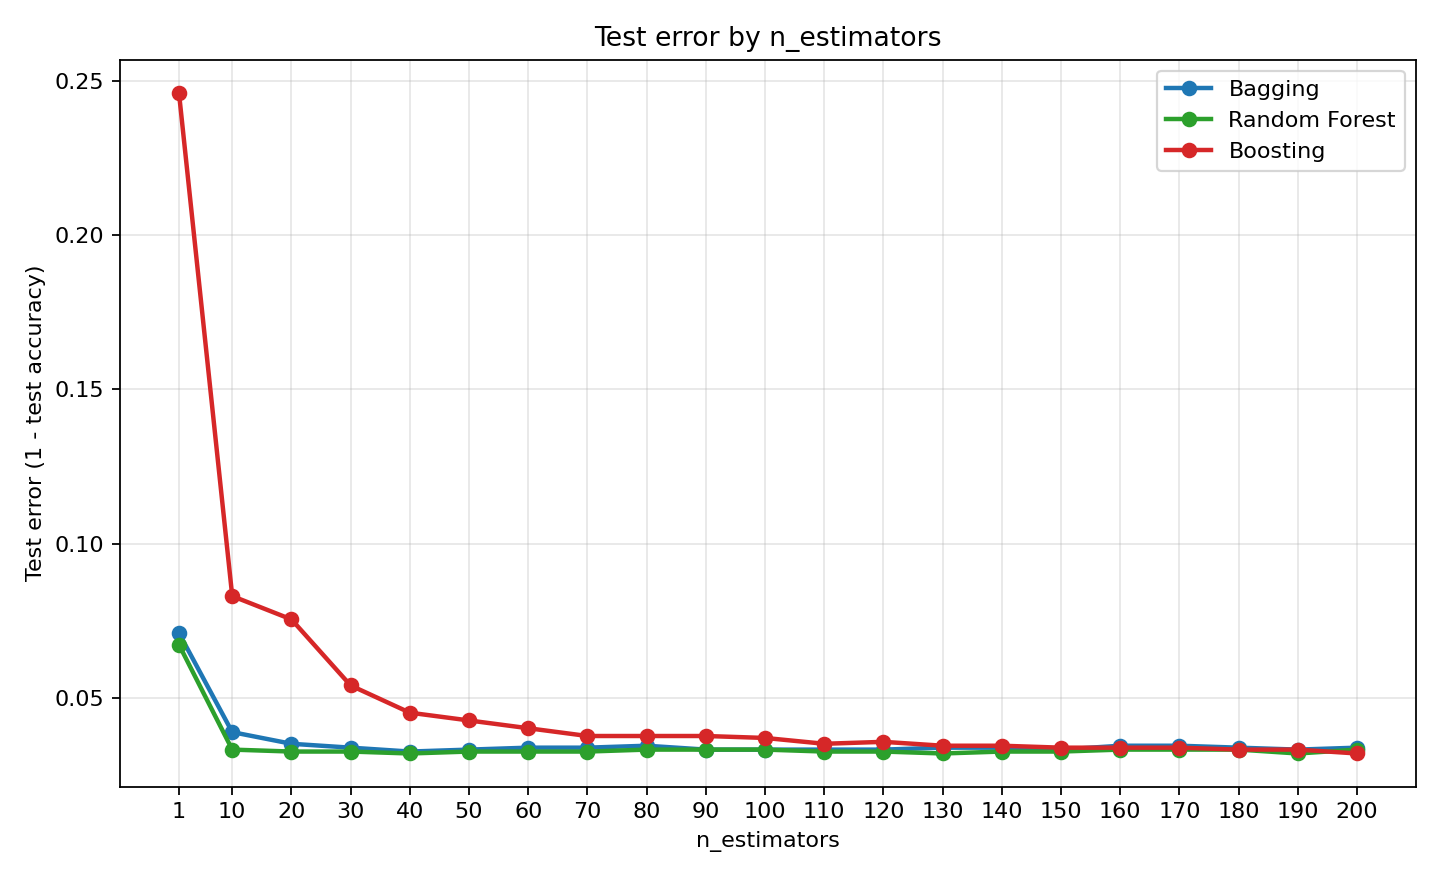
\includegraphics[width=0.92\textwidth]{q6_ensemble_n_estimators_error.png}
\caption{Test error των Bagging, Random Forest και Boosting συναρτήσει του αριθμού εκτιμητών.}
\label{fig:q6-n-estimators}
\end{figure}

\subsection{Σχολιασμός ανά μέθοδο}

\subsubsection*{Bagging}

Για το Bagging, το test error μειώνεται από 0.0711 όταν υπάρχει μόνο ένας
εκτιμητής σε 0.0390 για 10 εκτιμητές και σε 0.0352 για 20 εκτιμητές. Μετά από
περίπου 40 εκτιμητές, η καμπύλη σταθεροποιείται κοντά στο 0.033--0.034. Το
χαμηλότερο test error που παρατηρήθηκε ήταν 0.0327 για
\code{n\_estimators=40}.

Άρα η μεγάλη βελτίωση εμφανίζεται στην αρχή, όταν περνάμε από ένα δέντρο σε
ένα μικρό ensemble. Η περαιτέρω αύξηση των εκτιμητών προσφέρει μικρή ή
μηδενική βελτίωση.

\subsubsection*{Random Forest}

Το Random Forest φτάνει πολύ γρήγορα σε χαμηλό test error. Ήδη για
\code{n\_estimators=10} το test error είναι 0.0334, δηλαδή σχεδόν ίδιο με τις
μεγαλύτερες τιμές του αριθμού εκτιμητών. Το χαμηλότερο test error ήταν:
\[
    0.0321,
\]
και εμφανίστηκε για \code{n\_estimators=40}, \code{130} και \code{190}.

Η καμπύλη του Random Forest είναι η πιο σταθερή από τις τρεις. Αυτό δείχνει
ότι η τυχαιοποίηση στα χαρακτηριστικά, σε συνδυασμό με το ensemble δέντρων,
οδηγεί σε πολύ καλή απόδοση ακόμη και με σχετικά μικρό αριθμό δέντρων.

\subsubsection*{Boosting}

Το Boosting έχει διαφορετική συμπεριφορά. Για \code{n\_estimators=1}, το test
error είναι πολύ υψηλό, ίσο με 0.2461. Αυτό είναι αναμενόμενο, επειδή κάθε
επιμέρους μοντέλο είναι πολύ απλό δέντρο βάθους 1. Καθώς αυξάνεται ο αριθμός
των εκτιμητών, το test error μειώνεται σταδιακά:
\[
    0.0831 \text{ για } n=10, \qquad
    0.0453 \text{ για } n=40, \qquad
    0.0321 \text{ για } n=200.
\]

Σε αντίθεση με το Bagging και το Random Forest, το Boosting συνεχίζει να
βελτιώνεται μέχρι τις μεγαλύτερες τιμές του \code{n\_estimators}. Αυτό
οφείλεται στη σειριακή φύση της μεθόδου: κάθε νέο ασθενές μοντέλο προστίθεται
ώστε να διορθώσει σταδιακά τα σφάλματα του προηγούμενου συνόλου μοντέλων.

\subsection{Συμπέρασμα ερωτήματος 6}

Συνολικά, οι τρεις μέθοδοι καταλήγουν σε πολύ κοντινή απόδοση για μεγάλες τιμές
του \code{n\_estimators}. Το Bagging και το Random Forest σταθεροποιούνται πιο
γρήγορα, ενώ το Boosting χρειάζεται περισσότερους εκτιμητές για να φτάσει στο
ίδιο επίπεδο απόδοσης. Για \code{n\_estimators=200}, το χαμηλότερο test error
επιτυγχάνεται από το Boosting:
\[
    \text{Boosting test error}=0.0321.
\]

%=============================================================================
\section{Ερώτημα 7: Hyperparameter tuning και τελική σύγκριση}
%=============================================================================

Στο έβδομο ερώτημα πραγματοποιήθηκε βελτιστοποίηση υπερπαραμέτρων για κάθε μία
από τις τέσσερις μεθόδους. Η βελτιστοποίηση έγινε μόνο στο training set, με
Grid Search και 5-fold stratified cross-validation.

Η χρήση stratified cross-validation είναι σημαντική επειδή οι δύο κλάσεις δεν
είναι ισορροπημένες. Με αυτόν τον τρόπο κάθε fold διατηρεί περίπου την ίδια
αναλογία κόκκινων και λευκών κρασιών.

\subsection{Διαδικασία tuning}

Για κάθε μοντέλο ορίστηκε πλέγμα υποψήφιων τιμών υπερπαραμέτρων. Για κάθε
συνδυασμό υπερπαραμέτρων υπολογίστηκε η μέση ακρίβεια cross-validation. Στη
συνέχεια επιλέχθηκε ο συνδυασμός με τη μεγαλύτερη μέση CV accuracy. Το
βέλτιστο μοντέλο επανεκπαιδεύτηκε στο training set και αξιολογήθηκε μία φορά
στο test set.

Συνοπτικά, η διαδικασία ήταν:

\begin{enumerate}[nosep]
    \item Διαχωρισμός δεδομένων σε training/test με \code{random\_state=6931}.
    \item Ορισμός πλέγματος υπερπαραμέτρων για κάθε μέθοδο.
    \item Εφαρμογή \code{GridSearchCV} με 5-fold stratified CV στο training set.
    \item Επιλογή καλύτερων υπερπαραμέτρων βάσει CV accuracy.
    \item Αξιολόγηση του tuned μοντέλου στο test set.
\end{enumerate}

\subsection{Πλέγματα υπερπαραμέτρων}

\begin{table}[H]
\centering
\caption{Υπερπαράμετροι που εξετάστηκαν στη διαδικασία Grid Search.}
\small
\begin{tabular}{p{3.2cm}p{10.5cm}}
\toprule
\textbf{Μέθοδος} & \textbf{Υποψήφιες τιμές} \\
\midrule
Decision Tree &
\code{criterion}: gini, entropy;
\code{max\_depth}: 1, 2, 3, 4, 5, 6, 8, 10, 12, None;
\code{min\_samples\_leaf}: 1, 2, 5, 10 \\
\addlinespace
Bagging &
\code{n\_estimators}: 50, 100, 200;
\code{max\_samples}: 0.7, 1.0;
\code{max\_features}: 0.7, 1.0;
\code{estimator\_\_max\_depth}: None, 6 \\
\addlinespace
Random Forest &
\code{n\_estimators}: 50, 100, 200;
\code{max\_features}: 3, 5, sqrt;
\code{max\_depth}: None, 6, 10;
\code{min\_samples\_leaf}: 1, 2 \\
\addlinespace
Boosting &
\code{n\_estimators}: 50, 100, 200;
\code{learning\_rate}: 0.05, 0.1, 0.2;
\code{max\_depth}: 1, 2;
\code{subsample}: 0.8, 1.0 \\
\bottomrule
\end{tabular}
\end{table}

\subsection{Βέλτιστες υπερπαράμετροι και tuned test accuracy}

\begin{table}[H]
\centering
\caption{Βέλτιστες υπερπαράμετροι και ακρίβεια των tuned μοντέλων.}
\small
\begin{tabular}{p{2.8cm}p{7.9cm}rr}
\toprule
\textbf{Μέθοδος} & \textbf{Βέλτιστες υπερπαράμετροι} & \textbf{CV Acc.} & \textbf{Test Acc.} \\
\midrule
Decision Tree &
\code{criterion=gini}, \code{max\_depth=6}, \code{min\_samples\_leaf=1} &
0.9574 & 0.9654 \\
\addlinespace
Bagging &
\code{estimator\_\_max\_depth=6}, \code{max\_features=0.7}, \code{max\_samples=1.0}, \code{n\_estimators=50} &
0.9679 & 0.9729 \\
\addlinespace
Random Forest &
\code{max\_depth=10}, \code{max\_features=3}, \code{min\_samples\_leaf=1}, \code{n\_estimators=100} &
0.9690 & 0.9717 \\
\addlinespace
Boosting &
\code{learning\_rate=0.1}, \code{max\_depth=2}, \code{n\_estimators=200}, \code{subsample=1.0} &
0.9665 & 0.9692 \\
\bottomrule
\end{tabular}
\end{table}

\subsection{Σύγκριση untuned και tuned μοντέλων}

\begin{table}[H]
\centering
\caption{Σύγκριση αρχικών και βελτιστοποιημένων μοντέλων.}
\small
\begin{tabular}{@{}lccccc@{}}
\toprule
\textbf{Μέθοδος} &
\textbf{\shortstack{Untuned\\Acc.}} &
\textbf{\shortstack{Tuned\\Acc.}} &
\textbf{Μεταβολή} &
\textbf{\shortstack{Untuned\\Error}} &
\textbf{\shortstack{Tuned\\Error}} \\
\midrule
Decision Tree & 0.9339 & 0.9654 & +0.0315 & 0.0661 & 0.0346 \\
Bagging       & 0.9660 & 0.9729 & +0.0069 & 0.0340 & 0.0271 \\
Random Forest & 0.9666 & 0.9717 & +0.0050 & 0.0334 & 0.0283 \\
Boosting      & 0.9679 & 0.9692 & +0.0013 & 0.0321 & 0.0308 \\
\bottomrule
\end{tabular}
\end{table}

\subsection{Πίνακες σύγχυσης tuned μοντέλων}

\begin{table}[H]
\centering
\caption{Πίνακες σύγχυσης για τα βελτιστοποιημένα μοντέλα.}
\small
\begin{tabular}{lrrrr}
\toprule
\textbf{Μέθοδος} & \textbf{TN} & \textbf{FP} & \textbf{FN} & \textbf{TP} \\
\midrule
Decision Tree & 367 & 24 & 31 & 1167 \\
Bagging       & 370 & 21 & 22 & 1176 \\
Random Forest & 368 & 23 & 22 & 1176 \\
Boosting      & 364 & 27 & 22 & 1176 \\
\bottomrule
\end{tabular}
\end{table}

\subsection{Σχολιασμός της επίδρασης του tuning}

Η διαδικασία tuning βελτίωσε την απόδοση όλων των μοντέλων. Η μεγαλύτερη
βελτίωση παρατηρήθηκε στο απλό δέντρο ταξινόμησης. Το αρχικό δέντρο είχε
\code{max\_depth=2} και test accuracy 0.9339. Μετά το tuning, το βέλτιστο
βάθος έγινε \code{max\_depth=6}, και η test accuracy αυξήθηκε σε 0.9654. Η
βελτίωση αυτή είναι σημαντική:
\[
    0.9654 - 0.9339 = 0.0315.
\]
Αυτό δείχνει ότι το αρχικό δέντρο ήταν υπερβολικά απλό και δεν αξιοποιούσε
πλήρως την πληροφορία των δεδομένων.

Στις ensemble μεθόδους, η βελτίωση ήταν μικρότερη αλλά υπαρκτή. Αυτό είναι
αναμενόμενο, διότι τα αρχικά ensemble μοντέλα είχαν ήδη πολύ υψηλή ακρίβεια.
Το Bagging βελτιώθηκε από 0.9660 σε 0.9729. Το Random Forest βελτιώθηκε από
0.9666 σε 0.9717. Το Boosting βελτιώθηκε από 0.9679 σε 0.9692.

Η μικρότερη βελτίωση εμφανίζεται στο Boosting. Αυτό δεν σημαίνει ότι το
Boosting είναι αδύναμο μοντέλο· αντίθετα, το αρχικό Boosting ήταν ήδη το
καλύτερο από τα untuned μοντέλα. Επομένως υπήρχε μικρότερο περιθώριο
βελτίωσης μέσω tuning.

\subsection{Καλύτερη μέθοδος ταξινόμησης}

Αν ληφθούν υπόψη μόνο τα αρχικά μοντέλα των ερωτημάτων 1--4, η καλύτερη
ακρίβεια προκύπτει από το Boosting:

\begin{table}[H]
\centering
\caption{Κατάταξη αρχικών μοντέλων ως προς test accuracy.}
\begin{tabular}{lr}
\toprule
\textbf{Μέθοδος} & \textbf{Untuned Test Accuracy} \\
\midrule
Boosting & 0.9679 \\
Random Forest & 0.9666 \\
Bagging & 0.9660 \\
Decision Tree & 0.9339 \\
\bottomrule
\end{tabular}
\end{table}

Μετά τη βελτιστοποίηση, η καλύτερη ακρίβεια προκύπτει από το Bagging:

\begin{table}[H]
\centering
\caption{Κατάταξη tuned μοντέλων ως προς test accuracy.}
\begin{tabular}{lr}
\toprule
\textbf{Μέθοδος} & \textbf{Tuned Test Accuracy} \\
\midrule
Bagging & 0.9729 \\
Random Forest & 0.9717 \\
Boosting & 0.9692 \\
Decision Tree & 0.9654 \\
\bottomrule
\end{tabular}
\end{table}

Συνολικά, η καλύτερη μέθοδος ταξινόμησης είναι το tuned Bagging, καθώς
πετυχαίνει τη μεγαλύτερη ακρίβεια στο test set:
\[
    \text{Test Accuracy}=0.9729
\]
και το μικρότερο test error:
\[
    \text{Test Error}=0.0271.
\]

Η διαφορά του tuned Bagging από το tuned Random Forest είναι μικρή
($0.9729$ έναντι $0.9717$), επομένως και οι δύο μέθοδοι έχουν πρακτικά πολύ
καλή απόδοση. Ωστόσο, με βάση το κριτήριο που ζητείται στην εργασία, δηλαδή
την test accuracy, το Bagging είναι το καλύτερο μοντέλο.

%=============================================================================
\section{Συνολικά συμπεράσματα}
%=============================================================================

Η πρόβλεψη του τύπου κρασιού με βάση τα φυσικοχημικά χαρακτηριστικά είναι ένα
πρόβλημα στο οποίο οι μέθοδοι δέντρων και ensemble ταξινομητών αποδίδουν πολύ
καλά. Ακόμη και το απλό δέντρο βάθους 2 πετυχαίνει accuracy 0.9339, γεγονός
που δείχνει ότι οι δύο κατηγορίες κρασιού διαχωρίζονται αρκετά καλά από
ορισμένες βασικές μεταβλητές, όπως τα θειώδη και τα χλωρίδια.

Οι ensemble μέθοδοι βελτιώνουν αισθητά την απόδοση. Το Bagging και το Random
Forest μειώνουν τη διακύμανση συνδυάζοντας πολλά δέντρα, ενώ το Boosting
χτίζει διαδοχικά ένα ισχυρό μοντέλο από απλούς ασθενείς ταξινομητές. Στα
αρχικά μοντέλα, το Boosting είχε την καλύτερη ακρίβεια, ίση με 0.9679.

Η μελέτη του βάθους του δέντρου έδειξε ότι η αύξηση της πολυπλοκότητας
βελτιώνει το μοντέλο μέχρι ένα σημείο. Το καλύτερο βάθος ήταν 6, ενώ για
μεγαλύτερα βάθη το test error άρχισε να αυξάνεται, ένδειξη υπερπροσαρμογής.
Αντίστοιχα, η μελέτη του \code{n\_estimators} έδειξε ότι Bagging και Random
Forest σταθεροποιούνται γρήγορα, ενώ το Boosting χρειάζεται περισσότερους
εκτιμητές για να φτάσει στη βέλτιστη απόδοση.

Τέλος, το hyperparameter tuning βελτίωσε όλα τα μοντέλα. Η μεγαλύτερη
βελτίωση εμφανίστηκε στο απλό δέντρο, ενώ στις ensemble μεθόδους οι βελτιώσεις
ήταν μικρότερες επειδή οι αρχικές επιδόσεις ήταν ήδη υψηλές. Το καλύτερο
τελικό μοντέλο ήταν το tuned Bagging, με test accuracy 0.9729.

%=============================================================================
\appendix
\section{Αρχεία υλοποίησης}
%=============================================================================

Η ανάλυση υλοποιήθηκε με τα εξής scripts:

\begin{itemize}[nosep]
    \item \code{q1\_decision\_tree.py}
    \item \code{q2\_bagging.py}
    \item \code{q3\_random\_forest.py}
    \item \code{q4\_boosting.py}
    \item \code{q5\_tree\_depth\_error.py}
    \item \code{q6\_ensemble\_n\_estimators\_error.py}
    \item \code{q7\_hyperparameter\_tuning.py}
\end{itemize}

Τα βασικά παραγόμενα αρχεία αποτελεσμάτων είναι:

\begin{itemize}[nosep]
    \item \code{q5\_tree\_depth\_error.png}
    \item \code{q6\_ensemble\_n\_estimators\_error.png}
    \item \code{q7\_hyperparameter\_tuning\_summary.csv}
    \item \code{q7\_final\_comparison.md}
\end{itemize}

\end{document}
